\documentclass[12pt, a4paper]{book}

\usepackage[T1]{fontenc}
\usepackage[utf8]{inputenc}
\usepackage[charter, cal=cmcal]{mathdesign}
\usepackage[scaled=0.92]{helvet}
\usepackage{geometry}
\geometry{a4paper, top=30mm, bottom=30mm, inner=32mm, outer=25mm, marginparwidth=18mm}

\usepackage{amsmath, amsthm}
\usepackage[version=4]{mhchem}
\usepackage{graphicx}
\usepackage{xcolor}
\usepackage{tikz}
\usetikzlibrary{arrows.meta, shapes.geometric, positioning, calc, backgrounds}
\usepackage{pgfplots}
\pgfplotsset{compat=1.18}
\usepackage{tcolorbox}
\tcbuselibrary{skins, breakable, theorems}
\usepackage{titlesec}
\usepackage{fancyhdr}
\usepackage{enumitem}
\usepackage{booktabs}
\usepackage{array}
\usepackage{parskip}
\usepackage{siunitx}
\usepackage[colorlinks=true, linkcolor=BrickRed,
            urlcolor=NavyBlue, citecolor=ForestGreen]{hyperref}

% ── Colours (Charcoal / Royal Blue) ──────────────────────────────────────────
\definecolor{JourneyColor}{HTML}{0F172A}
\definecolor{ModuleColor}{HTML}{2563EB}
\definecolor{PuzzleColor}{HTML}{D97706}
\definecolor{DiscoveryColor}{HTML}{3B82F6}
\definecolor{WarningColor}{HTML}{991B1B}
\definecolor{ProblemColor}{HTML}{6B21A8}
\definecolor{ReflectColor}{HTML}{0D9488}
\definecolor{HistoryColor}{HTML}{78350F}

% ── Boxes ─────────────────────────────────────────────────────────────────────
\newtcolorbox{puzzlebox}[1][]{enhanced,breakable,
  colback=PuzzleColor!6,colframe=PuzzleColor,fonttitle=\bfseries\sffamily,
  title={The Puzzle},attach boxed title to top left={yshift=-2mm,xshift=6mm},
  boxed title style={colback=PuzzleColor},borderline west={3pt}{0pt}{PuzzleColor},#1}

\newtcolorbox{discoverybox}[1][]{enhanced,breakable,
  colback=DiscoveryColor!8,colframe=DiscoveryColor,fonttitle=\bfseries\sffamily,
  title={Discovery},attach boxed title to top left={yshift=-2mm,xshift=6mm},
  boxed title style={colback=DiscoveryColor},borderline west={3pt}{0pt}{DiscoveryColor},#1}

\newtcolorbox{problembox}[1][]{enhanced,breakable,
  colback=ProblemColor!5,colframe=ProblemColor,fonttitle=\bfseries\sffamily,
  title={Problems},attach boxed title to top left={yshift=-2mm,xshift=6mm},
  boxed title style={colback=ProblemColor},borderline west={3pt}{0pt}{ProblemColor},#1}

\newtcolorbox{deepbox}[1][]{enhanced,breakable,
  colback=JourneyColor!5,colframe=JourneyColor,fonttitle=\bfseries\sffamily,
  title={Deep Problems},attach boxed title to top left={yshift=-2mm,xshift=6mm},
  boxed title style={colback=JourneyColor},borderline west={4pt}{0pt}{JourneyColor},#1}

\newtcolorbox{historybox}[1][]{enhanced,breakable,
  colback=HistoryColor!7,colframe=HistoryColor!60,fonttitle=\bfseries\sffamily\small,
  title={History Note},attach boxed title to top left={yshift=-2mm,xshift=6mm},
  boxed title style={colback=HistoryColor!80},#1}

\newtcolorbox{reflectionbox}[1][]{enhanced,breakable,
  colback=ReflectColor!6,colframe=ReflectColor,fonttitle=\bfseries\sffamily,
  title={Reflection},attach boxed title to top left={yshift=-2mm,xshift=6mm},
  boxed title style={colback=ReflectColor},borderline west={3pt}{0pt}{ReflectColor},#1}

\newtcolorbox{namedconcept}[2][]{enhanced,
  colback=ModuleColor!6,colframe=ModuleColor,fonttitle=\bfseries\sffamily\large,
  title={#2},attach boxed title to top left={yshift=-2mm,xshift=6mm},
  boxed title style={colback=ModuleColor},#1}

% ── Section formatting ────────────────────────────────────────────────────────
\titleformat{\chapter}[display]
  {\normalfont\sffamily\huge\bfseries\color{JourneyColor}}
  {\textcolor{JourneyColor!60}{\chaptertitlename\ \thechapter}}{10pt}{\Huge}
  [\vspace{2pt}\textcolor{JourneyColor}{\titlerule[1.5pt]}]
\titleformat{\section}
  {\normalfont\sffamily\Large\bfseries\color{ModuleColor}}
  {\thesection}{1em}{}[\textcolor{ModuleColor!40}{\titlerule[0.6pt]}]
\titleformat{\subsection}
  {\normalfont\sffamily\large\bfseries\color{JourneyColor!80}}{\thesubsection}{1em}{}
\titleformat{\subsubsection}
  {\normalfont\sffamily\normalsize\bfseries}{\thesubsubsection}{1em}{}

\pagestyle{fancy}
\fancyhf{}
\fancyhead[LE]{\small\sffamily\textcolor{JourneyColor}{\leftmark}}
\fancyhead[RO]{\small\sffamily\textcolor{ModuleColor}{\rightmark}}
\fancyfoot[C]{\small\thepage}
\renewcommand{\headrulewidth}{0.4pt}

\newcommand{\newterm}[1]{\textit{\textcolor{DiscoveryColor}{#1}}}
\newcommand{\important}[1]{\textcolor{ModuleColor}{\textbf{#1}}}

\begin{document}

\setcounter{chapter}{4}
\chapter[Journey 5 --- Algorithms, Data Structures, and Optimization]
        {Journey Five\\[8pt]
         \textcolor{ModuleColor}{\large Algorithms, Data Structures, and Optimization}}
\setcounter{section}{2}

\section{Module 5.3 --- Graph Algorithms and Network Flow}
\label{sec:mod5.3}

\subsection*{Motivation}

We completed in Module 5.2 the advanced structures for dynamic data storage, studying Red-Black trees and Universal Hashing.
But data in physical networks is rarely isolated.
Information exists as networks of interconnected nodes.
We must study the topology of connection.

In this module, we formalize the mathematical analysis of **Graphs**.
We will study pathfinding, contrasting Dijkstra's greedy priority queue with the Bellman-Ford cycle-detection algorithm.
Then, we will analyze flow networks, investigating how the Ford-Fulkerson algorithm maximizes transfer capacities.
Finally, we will prove the **Max-Flow Min-Cut Theorem**, demonstrating a deep duality between network capacity and bottleneck cuts.

\subsection{The Network Routing Bottleneck}

We investigate pathfinding constraints and maximum capacity throughput.

\begin{puzzlebox}
\textbf{The Fiber Graph.}

Suppose a communication network is modeled as a directed graph $G = (V, E)$, where vertices are routers and edges are optical fibers.
Each fiber has:
* A transmission delay (edge weight $w(u, v) \ge 0$).
* A maximum bandwidth capacity (edge capacity $c(u, v) > 0$).
\begin{enumerate}[label=(\alph*), leftmargin=*]
  \item If we want to send a packet from source $s$ to sink $t$ with minimum delay, we use **Dijkstra's Algorithm**.
        Suppose an edge has a negative delay (due to a clock sync offset or routing incentive).
        Explain why Dijkstra's greedy assumption fails when negative edge weights are present.
  \item If we want to maximize the volume of data sent simultaneously from $s$ to $t$, we model it as a **Flow Network**.
        Write down the two fundamental constraints of a valid network flow:
        * **Capacity Constraint:** How does flow $f(u, v)$ relate to capacity $c(u, v)$?
        * **Flow Conservation:** What must be true of the total flow entering and exiting any node other than $s$ and $t$?
  \item We define a **Cut $(S, T)$** as a partition of $V$ such that $s \in S$ and $t \in T$.
        Explain why the total net flow crossing any cut must be exactly equal to the total flow leaving the source $s$.
        How does the capacity of the *minimum* capacity bottleneck cut bound the maximum possible flow from $s$ to $t$?
\end{enumerate}
\end{puzzlebox}

\subsection{Shortest Paths: Dijkstra and Bellman-Ford}

We study greedy path relaxation and cycle-detecting dynamic programming.

\begin{namedconcept}{Dijkstra's Shortest Path Algorithm}
Let $G = (V, E)$ be a weighted graph with non-negative weights $w(u, v) \ge 0$.
Dijkstra's algorithm maintains a set $S$ of vertices whose final shortest-path weights from $s$ have been determined.
It repeatedly selects the vertex $u \in V \setminus S$ with the minimum shortest-path estimate $d[u]$, inserts $u$ into $S$, and relaxes all edges leaving $u$:
\[
  \text{Relax}(u, v, w) \quad:\quad \text{if } d[v] > d[u] + w(u, v) \text{ then } d[v] := d[u] + w(u, v)
\]
\end{namedconcept}

\begin{explobox}
If negative edge weights are present, we must use the **Bellman-Ford Algorithm**, which relaxes all edges in the graph $V-1$ times:
\begin{enumerate}[label=(\alph*), leftmargin=*]
  \item Prove that if a graph contains no negative-weight cycles, any shortest path contains at most $V-1$ edges.
        Why does this guarantee that $V-1$ passes of relaxation are sufficient to find the shortest path?
  \item If we run relaxation a $V$-th time and any distance estimate decreases ($d[v] > d[u] + w(u, v)$), what does this reveal about the graph?
  \item Compare the time complexity of Dijkstra's algorithm (using a binary heap priority queue) to the Bellman-Ford algorithm. What is the efficiency cost of supporting negative weights?
\end{enumerate}
\end{explobox}

\subsection{Flow Networks and the Max-Flow Min-Cut Theorem}

We study flow augmentation in residual networks and prove bottleneck dualities.

\begin{explobox}
The **Ford-Fulkerson Method** finds the maximum flow by working on the **Residual Network** $G_f = (V, E_f)$.
* The residual capacity is defined as:
  \[
    c_f(u, v) \;=\; c(u, v) - f(u, v) \quad \text{for forward edges}
  \]
  \[
    c_f(u, v) \;=\; f(v, u) \quad \text{for backward edges}
  \]
* An **Augmenting Path** $p$ is a simple path from $s$ to $t$ in $G_f$ where $c_f(u, v) > 0$ for all edges on $p$.
\begin{enumerate}[label=(\alph*), leftmargin=*]
  \item Why do we include backward edges with capacity $c_f(u, v) = f(v, u)$ in the residual network? (How does this allow the algorithm to "undo" bad flow assignments made in earlier steps?)
  \item The **Max-Flow Min-Cut Theorem** states that the value of a maximum flow is exactly equal to the capacity of the minimum cut.
        Let $f^*$ be a maximum flow.
        Construct the minimum cut $(S, T)$ by defining $S$ as the set of vertices reachable from $s$ in the final residual graph $G_{f^*}$.
        Show why no residual capacity can leave $S$, and conclude that $f^*$ equals the capacity of the cut $(S, T)$.
\end{enumerate}
\end{explobox}

\newpage

% ─── Section: Discovery ──────────────────────────────────────────────────────
\section{Part 3 --- Discovery}

\begin{discoverybox}
\textbf{What have we built?}

\textbf{First.} Dijkstra's algorithm uses a greedy priority queue to resolve shortest paths in $O((V+E) \log V)$ time under non-negative weights.

\textbf{Second.} Bellman-Ford uses $V-1$ iterations of edge relaxations to solve shortest paths under negative weights and identify negative-weight cycles.

\textbf{Third.} Residual networks map both forward excess capacities and backward flow redirect limits, enabling iterative flow optimizations.

\textbf{Fourth.} The Max-Flow Min-Cut Theorem proves that the maximum flow volume is mathematically bounded and equal to the capacity of the minimum cut.
\end{discoverybox}

\newpage

% ─── Section: Naming Concepts ────────────────────────────────────────────────
\section{Part 4 --- What This Is Called}

\begin{namedconcept}{Graph parameters}
* **Relaxation:** The process of testing if we can improve the shortest path to vertex $v$ by going through vertex $u$.
* **Negative-Weight Cycle:** A cycle in a weighted graph whose total edge weight sum is negative, causing shortest paths to approach $-\infty$.
* **Flow Network:** A directed graph where edges represent capacities for routing commodity flow.
* **Residual Network ($G_f$):** A representation of a flow network showing remaining available capacities and redirect limits.
* **Min-Cut:** The partition of a graph separating source and sink that minimizes the sum of edge capacities crossing the cut.
\end{namedconcept}

\newpage

% ─── Section: Solved Exercises ───────────────────────────────────────────────
\section{Part 5 --- Solved Exercises}

\begin{problembox}
\begin{enumerate}[label=\textbf{E\arabic*.}]
  \item \textbf{Dijkstra Execution on Weighted Graph.}
  
        Trace Dijkstra's algorithm to find the shortest paths from source $s$ to all other nodes in the following directed graph:
        \begin{center}
        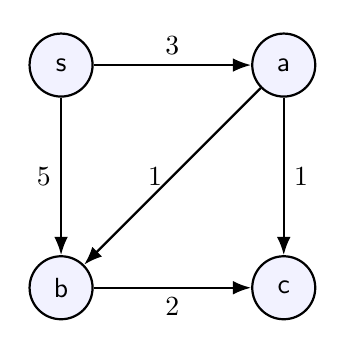
\begin{tikzpicture}[
          >=Latex, node distance=2cm,
          node/.style={circle, draw, thick, fill=blue!5, minimum size=0.8cm, font=\sffamily}
        ]
          \node[node] (s) {s};
          \node[node, right=of s] (a) {a};
          \node[node, below=of s] (b) {b};
          \node[node, right=of b] (c) {c};
          
          \draw[->, thick] (s) -- node[above] {3} (a);
          \draw[->, thick] (s) -- node[left] {5} (b);
          \draw[->, thick] (a) -- node[right] {1} (c);
          \draw[->, thick] (b) -- node[below] {2} (c);
          \draw[->, thick] (a) -- node[left] {1} (b);
        \end{tikzpicture}
        \end{center}
        
        \textbf{Solution:}
        1. **Initialization:**
           Set $d[s] = 0$, and $d[a] = d[b] = d[c] = \infty$.
           Visited set $S = \emptyset$. Priority queue $Q = \{ (s,0), (a,\infty), (b,\infty), (c,\infty) \}$.
           
        2. **Iteration 1:**
           Extract minimum node $u = s$ ($d[s] = 0$). Add to $S = \{s\}$.
           Relax outgoing edges from $s$:
           * Edge $(s, a)$ with weight 3: $d[a] > d[s] + 3 \implies d[a] := 3$.
           * Edge $(s, b)$ with weight 5: $d[b] > d[s] + 5 \implies d[b] := 5$.
           Queue state: $Q = \{ (a,3), (b,5), (c,\infty) \}$.
           
        3. **Iteration 2:**
           Extract minimum node $u = a$ ($d[a] = 3$). Add to $S = \{s, a\}$.
           Relax outgoing edges from $a$:
           * Edge $(a, b)$ with weight 1: $d[b] > d[a] + 1 \implies d[b] := 3 + 1 = 4$.
           * Edge $(a, c)$ with weight 1: $d[c] > d[a] + 1 \implies d[c] := 3 + 1 = 4$.
           Queue state: $Q = \{ (b,4), (c,4) \}$.
           
        4. **Iteration 3:**
           Extract minimum node $u = b$ ($d[b] = 4$). Add to $S = \{s, a, b\}$.
           Relax outgoing edges from $b$:
           * Edge $(b, c)$ with weight 2: $d[c] > d[b] + 2 \implies 4 > 4 + 2$ (no change).
           Queue state: $Q = \{ (c,4) \}$.
           
        5. **Iteration 4:**
           Extract minimum node $u = c$ ($d[c] = 4$). Add to $S = \{s, a, b, c\}$.
           Queue is empty.
           
        Final shortest path estimates: $d[s] = 0, d[a] = 3, d[b] = 4, d[c] = 4$.
        
  \item \textbf{Failure of Dijkstra's Algorithm with Negative Weights.}
  
        Provide a concrete 3-node graph showing that Dijkstra's algorithm can yield incorrect shortest-path weights when negative edge weights are present.
        
        \textbf{Solution:}
        Consider the following directed graph:
        \begin{center}
        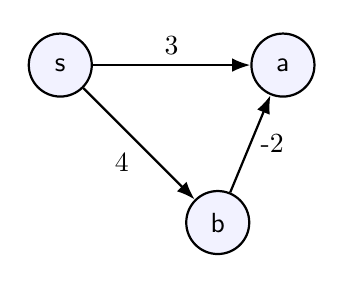
\begin{tikzpicture}[
          >=Latex, node distance=2cm,
          node/.style={circle, draw, thick, fill=blue!5, minimum size=0.8cm, font=\sffamily}
        ]
          \node[node] (s) {s};
          \node[node, right=of s] (a) {a};
          \node[node, below right=of s] (b) {b};
          
          \draw[->, thick] (s) -- node[above] {3} (a);
          \draw[->, thick] (s) -- node[below left] {4} (b);
          \draw[->, thick] (b) -- node[right] {-2} (a);
        \end{tikzpicture}
        \end{center}
        * **True shortest paths:**
          * Path $s \to a$ has weight $3$.
          * Path $s \to b \to a$ has weight $4 + (-2) = 2$.
          So the true shortest path distance to $a$ is $\delta(s, a) = 2$.
          
        * **Dijkstra's execution:**
          1. Initialize $d[s] = 0, d[a] = \infty, d[b] = \infty$.
          2. Extract $s$. Relax $(s, a)$ and $(s, b) \implies d[a] := 3, d[b] := 4$.
          3. Extract minimum node in queue: $a$ ($d[a] = 3$). Add $a$ to visited set $S = \{s, a\}$.
             At this point, Dijkstra locks in the shortest path to $a$ as $d[a] = 3$.
          4. Extract $b$ ($d[b] = 4$). Add $b$ to $S = \{s, a, b\}$.
             Relax outgoing edge $(b, a)$: $d[a] > d[b] + (-2) \implies 3 > 4 - 2 = 2$.
             But since $a$ has already been extracted and added to $S$, Dijkstra does not update $d[a]$ (or fails to propagate this update to children of $a$).
             
        Dijkstra's algorithm finishes with incorrect estimate $d[a] = 3$, whereas the true shortest path is $2$. This demonstrates the failure mode of the greedy assumption.
\end{enumerate}
\end{problembox}

\newpage

% ─── Section: Problems ───────────────────────────────────────────────────────
\section{Part 6 --- Problems}

\begin{problembox}
\begin{enumerate}[label=\textbf{P\arabic*.}]
  \item \textbf{Bellman-Ford and Negative Cycles.}
  
        Consider the directed graph containing a cycle:
        \begin{center}
        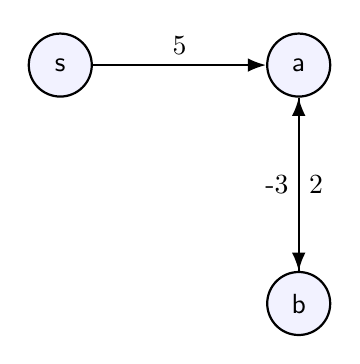
\begin{tikzpicture}[
          >=Latex, node distance=2.2cm,
          node/.style={circle, draw, thick, fill=blue!5, minimum size=0.8cm, font=\sffamily}
        ]
          \node[node] (s) {s};
          \node[node, right=of s] (a) {a};
          \node[node, below=of a] (b) {b};
          
          \draw[->, thick] (s) -- node[above] {5} (a);
          \draw[->, thick] (a) -- node[right] {2} (b);
          \draw[->, thick] (b) -- node[left] {-3} (a);
        \end{tikzpicture}
        \end{center}
        Note that the cycle $a \to b \to a$ has weight $2 + (-3) = -1$ (negative weight cycle).
        \begin{enumerate}[label=(\alph*)]
          \item Trace the distance estimates $d[s], d[a], d[b]$ through 3 complete passes of relaxation of the Bellman-Ford algorithm starting from $s$.
          \item Show the distance values on the 4th pass. Explain how the algorithm detects the presence of the negative cycle.
        \end{enumerate}

  \item \textbf{Ford-Fulkerson Augmenting Paths.}
  
        Trace the Ford-Fulkerson algorithm to find the maximum flow from $s$ to $t$ in the following flow network (numbers represent edge capacities):
        \begin{center}
        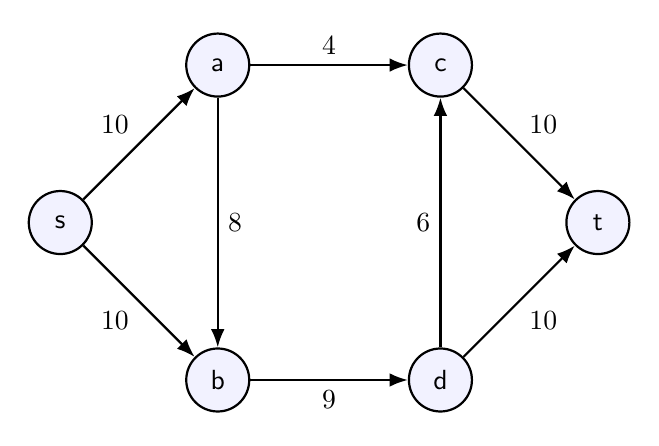
\begin{tikzpicture}[
          >=Latex, node distance=2cm,
          node/.style={circle, draw, thick, fill=blue!5, minimum size=0.8cm, font=\sffamily}
        ]
          \node[node] (s) {s};
          \node[node, above right=of s] (a) {a};
          \node[node, below right=of s] (b) {b};
          \node[node, right=of a] (c) {c};
          \node[node, right=of b] (d) {d};
          \node[node, below right=of c] (t) {t};
          
          \draw[->, thick] (s) -- node[above left] {10} (a);
          \draw[->, thick] (s) -- node[below left] {10} (b);
          \draw[->, thick] (a) -- node[above] {4} (c);
          \draw[->, thick] (a) -- node[right] {8} (b);
          \draw[->, thick] (b) -- node[below] {9} (d);
          \draw[->, thick] (d) -- node[left] {6} (c);
          \draw[->, thick] (c) -- node[above right] {10} (t);
          \draw[->, thick] (d) -- node[below right] {10} (t);
        \end{tikzpicture}
        \end{center}
        \begin{enumerate}[label=(\alph*)]
          \item List each chosen augmenting path, its bottleneck capacity, and update the residual network after each step.
          \item Specify the final maximum flow value.
          \item Identify the minimum cut $(S, T)$ corresponding to this maximum flow. List the vertices in sets $S$ and $T$.
        \end{enumerate}
\end{enumerate}
\end{problembox}

\newpage

% ─── Section: Deep Problems ──────────────────────────────────────────────────
\section{Part 7 --- Deep Problems}

\begin{deepbox}
\begin{enumerate}[label=\textbf{D\arabic*.}]
  \item \textbf{Correctness Proof of Dijkstra's Algorithm.}
  
        We prove that when a vertex $u$ is added to the set $S$ of visited vertices, the distance estimate $d[u]$ equals the true shortest-path distance $\delta(s, u)$ from the source.
        Assume that all edge weights are non-negative ($w(u, v) \ge 0$).
        
        We prove this by contradiction. Let $u$ be the *first* vertex added to $S$ such that $d[u] \neq \delta(s, u)$ at the time of insertion. Note that $u \neq s$ because $d[s] = \delta(s, s) = 0$ is correct.
        
        \begin{enumerate}[label=(\alph*)]
          \item Since $u \neq s$ and $s \in S$, there must exist a true shortest path $p$ from $s$ to $u$.
                As $p$ starts in $S$ and ends in $V \setminus S$, let $(x, y)$ be the first edge along path $p$ such that $x \in S$ and $y \in V \setminus S$.
                Explain why $d[x] = \delta(s, x)$ and why $d[y] = \delta(s, y)$ immediately after $x$ was added to $S$.
          \item Since $y$ lies on the shortest path $p$ from $s$ to $u$, and all edge weights are non-negative, prove the inequality:
                \[
                  \delta(s, y) \;\le\; \delta(s, u).
                \]
          \item Since $u$ was selected from $Q = V \setminus S$ before $y$, we must have had $d[u] \le d[y]$ at that step.
                Combine this with your results from (a) and (b) to show that:
                \[
                  d[u] \;\le\; d[y] \;=\; \delta(s, y) \;\le\; \delta(s, u).
                \]
                Conclude that $d[u] = \delta(s, u)$, contradicting the assumption that $d[u] \neq \delta(s, u)$.
        \end{enumerate}

  \item \textbf{Proof of the Max-Flow Min-Cut Theorem.}
  
        Let $f$ be a flow in a flow network $G = (V, E)$, and let $|f|$ be its value.
        We prove that the following three statements are equivalent:
        1. $f$ is a maximum flow in $G$.
        2. The residual network $G_f$ contains no augmenting paths.
        3. $|f| = c(S, T)$ for some cut $(S, T)$ of $G$.
        
        \begin{enumerate}[label=(\alph*)]
          \item Prove that $1 \implies 2$ by contradiction.
                *(Hint: Show that if there is an augmenting path in $G_f$, we can construct a new flow $f'$ such that $|f'| > |f|$).*
          \item Prove $2 \implies 3$. Let $G_f$ contain no augmenting paths.
                Define the set of vertices:
                \[
                  S \;=\; \{ v \in V \mid \text{there exists a path from } s \text{ to } v \text{ in } G_f \}.
                \]
                Let $T = V \setminus S$.
                Clearly $s \in S$. Since there is no augmenting path, explain why $t \in T$, making $(S, T)$ a valid cut.
                Prove that for any $u \in S$ and $v \in T$, we must have $f(u, v) = c(u, v)$ and $f(v, u) = 0$.
                Conclude that $|f| = c(S, T)$.
          \item Prove $3 \implies 1$ using the weak duality property: $|f| \le c(S, T)$ for any flow $f$ and any cut $(S, T)$.
        \end{enumerate}
\end{enumerate}
\end{deepbox}

\newpage

% ─── Section: Reflection ─────────────────────────────────────────────────────
\section{Part 8 --- Reflection}

\begin{reflectionbox}
\textbf{Conceptual Reflection}

Consider the following questions:
\begin{enumerate}
  \item **On the greedy assumption:** Dijkstra's algorithm relies on the greedy choice property: "the locally optimal step is globally optimal." This assumption fails when negative edge weights are present, requiring the global searches of Bellman-Ford. How does this illustrate the trade-off between *local optimization* and *global safety*?
  \item **On the duality of bottleneck:** The Max-Flow Min-Cut Theorem shows that the capacity of any complex network is entirely determined by its single most restricted bottleneck (the min-cut). How does this principle apply to other engineering systems (like compiler register spills, cache latencies, or CPU pipelines)?
  \item **On the abstraction of flow:** We modeled information flow as a continuous fluid moving through conduits. In reality, data packets are discrete and packet loss occurs. How does the continuous approximation of flow networks help us design routing protocols for discrete computer networks?
\end{enumerate}
\end{reflectionbox}

\medskip
\noindent\textbf{Looking ahead.}
Module~5.4 introduces **Dynamic Programming and Greedy Algorithms**. Having analyzed graph traversals and paths, we will study general techniques to solve complex optimization problems by breaking them down into overlapping subproblems or making sequential greedy choices.

\vspace{1.4cm}
\begin{center}
{\color{JourneyColor}\rule{0.5\linewidth}{0.8pt}}\\[6pt]
{\small\color{JourneyColor}\textit{End of Journey 5, Module 5.3 --- Graph Algorithms and Network Flow}}\\[4pt]
{\small\color{JourneyColor}Continue to: \textbf{Module 5.4 --- Dynamic Programming and Greedy Algorithms}}\\[6pt]
{\color{JourneyColor}\rule{0.5\linewidth}{0.8pt}}
\end{center}

\end{document}
